% ============================================================================
% Figure 3: Per-configuration SAT comparison (valid rate & timeout rate).
% Data source: paper/tables/table2_per_solver_breakdown.csv (audited against
% data/results/benchmark_sat_vs_nonsat.csv).
% Timeout rate computed as timeouts / attempted runs.
% Pairwise and binary each have 40 predeclared N=81 exclusions (attempted=80);
% commander has 1 live resource-guard rejection (attempted=120).
% ============================================================================
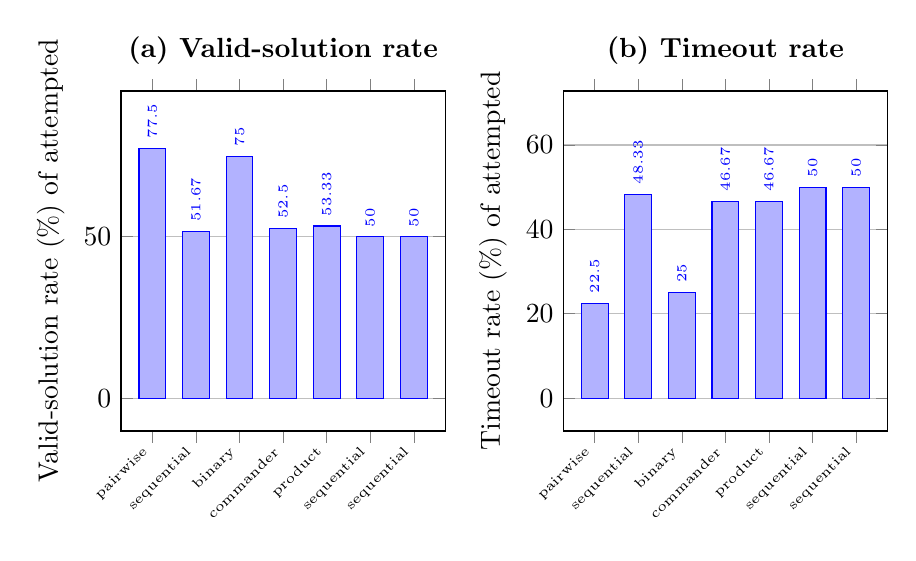
\begin{tikzpicture}
  % ---- Panel (a): valid-solution rate per SAT config ----
  \begin{axis}[
    name=plotA,
    ybar, bar width=0.34cm,
    symbolic x coords={
      pw_cad,seq_cad,bin_cad,com_cad,prod_cad,seq_glu,seq_mini
    },
    xtick=data,
    xticklabels={
      pairwise,sequential,binary,commander,product,sequential,sequential
    },
    xticklabel style={font=\tiny, rotate=45, anchor=east},
    xticklabel style={align=center},
    x tick label style={/pgf/number format/1000 sep={}},
    extra x tick labels={CaDiCaL,CaDiCaL,CaDiCaL,CaDiCaL,CaDiCaL,Glucose,MiniSat},
    extra x tick style={
      xticklabel style={font=\tiny, yshift=1.1em},
      xticklabel pos=right,
    },
    ylabel={Valid-solution rate (\%) of attempted},
    ymin=0, ymax=85,
    ymajorgrids=true,
    enlargelimits=0.12,
    legend style={at={(0.5,-0.42)}, anchor=north, font=\tiny},
    width=0.47\textwidth, height=5.9cm,
    title style={font=\bfseries},
    title={(a) Valid-solution rate},
    nodes near coords,
    nodes near coords align={vertical},
    every node near coord/.append style={font=\tiny\bfseries, rotate=90, anchor=west},
  ]
  \addplot coordinates {(pw_cad,77.50) (seq_cad,51.67) (bin_cad,75.00) (com_cad,52.50) (prod_cad,53.33) (seq_glu,50.00) (seq_mini,50.00)};
  \end{axis}

  % ---- Panel (b): timeout rate per SAT config ----
  \begin{axis}[
    at={(plotA.east)}, anchor=west, xshift=1.5cm,
    ybar, bar width=0.34cm,
    symbolic x coords={
      pw_cad,seq_cad,bin_cad,com_cad,prod_cad,seq_glu,seq_mini
    },
    xtick=data,
    xticklabels={
      pairwise,sequential,binary,commander,product,sequential,sequential
    },
    xticklabel style={font=\tiny, rotate=45, anchor=east},
    xticklabel style={align=center},
    x tick label style={/pgf/number format/1000 sep={}},
    extra x tick labels={CaDiCaL,CaDiCaL,CaDiCaL,CaDiCaL,CaDiCaL,Glucose,MiniSat},
    extra x tick style={
      xticklabel style={font=\tiny, yshift=1.1em},
      xticklabel pos=right,
    },
    ylabel={Timeout rate (\%) of attempted},
    ymin=0, ymax=65,
    ymajorgrids=true,
    enlargelimits=0.12,
    width=0.47\textwidth, height=5.9cm,
    title style={font=\bfseries},
    title={(b) Timeout rate},
    nodes near coords,
    nodes near coords align={vertical},
    every node near coord/.append style={font=\tiny\bfseries, rotate=90, anchor=west},
  ]
  \addplot coordinates {(pw_cad,22.50) (seq_cad,48.33) (bin_cad,25.00) (com_cad,46.67) (prod_cad,46.67) (seq_glu,50.00) (seq_mini,50.00)};
  \end{axis}
\end{tikzpicture}
